\input /Users/davidmcallester/Icloude/tex/SlidePreamble.tex
\input /Users/davidmcallester/Icloude/tex/preamble.tex

\begin{document}

{\Huge

  \centerline{\bf TTIC 31230, Fundamentals of Deep Learning}
  \bigskip
  \centerline{David McAllester, Autumn 2021}

  \vfill
  \centerline{\bf MuZero}
  \vfill
  \vfill

\slide{Action Planning for Atari}

{\bf Mastering Atari, Go, chess and shogi by planning with a learned model}, Schrittweiser et al., Nature 2020.

\vfill
While the paper describes a new system for board games (Chess, go and shogi) there is no significant improvement over AlphaZero for board games.

\vfill
The real innovation here is the generalization of AlphaZero to Atari games.

\vfill
I will focus on Atari Games.

\slide{Action Planning for Atari}

AlphaZero uses Monte-Carlo tree search (MCTS) to ``plan'' into the future.

\vfill
Planning requires a model of state transitions.

\vfill
Q-learning and advantage actor-critic do not require the ability to plan ahead (tree search). Previous Deep-Mind systems for Atari did not use MCTS to plan ahead.

\slide{Building a Model}

\vfill
MuZero for Atari sees the Atari screen and rewards during play but cannot see future screens when it does MCTS to plan for future outcomes.

\vfill
During MCTS MuZero uses a learned dynamic model --- an RNN $g_\Phi(s,a)$ for predicting reward and the next state.

\vfill
$$r^k,s^k = g_\Phi(s^{k-1},a^k)$$

\vfill
Given the RNN state model we can perform Monte Carlo tree search (MCTS) as in AlphaZero.

\slide{Training}

As in AlphaZero, we train a policy network and value network.

\vfill
But in MuZero we also train a model of state transitions and rewards to be used in MCTS.

\vfill
At the beginning of the each MCTS the state is initialized from the observed history of screen shots and actions taken.  This initialization network is also trained.

\slide{Training}

{\huge
The training loss function has the form

$$\Phi^* = \argmin_\Phi E_{s \sim \mathrm{Rollout}}\;{\cal L}^\pi(s) + {\cal L}^V(s) +{\cal L}^R(s) + c||\Phi||^2$$

\vfill
The rollouts are generated from the actions selected by MCTS and put in a replay buffer.

\vfill
The entries in the replay buffer have the form
$$s = \left[\;(o_1,a_1,\ldots,o_t,a_t);\;\;a_{t+1},\;r_{t+1},\ldots,a_{t+K},r_{t+K},v_{t+K+1}\;\right]$$

\vfill
where $a_t$ is the action taken at time $t$, $o_t$ is a screen shot at time, $r_t$ is the reward at time $t$ (from the actual game), and
$v_{t+K+1}$ is the discounted reward encountered from time $t+K+1$.
}
\slide{Training}

{\huge
$$\Phi^* = \argmin_\Phi E_{s \sim \mathrm{Rollout}}\;{\cal L}^\pi(s) + {\cal L}^V(s) +{\cal L}^R(s) + c||\Phi||^2$$

$$s  = \left[\;(o_1,a_1,\ldots,o_t,a_t);\;\;a_{t+1},\;r_{t+1},\ldots,a_{t+K},r_{t+K},v_{t+K+1}\;\right]$$
  
\vfill
${\cal L}^\pi$ trains the policy network to predict $a_{t+1}$ (a cross-entropy loss).

\vfill
${\cal L}^V$ trains the value network to predict $v_{t+K+1}$ (square loss).

\vfill
${\cal L}^R$ trains the reward network to predict each $r_{t+k}$ (square loss).

\vfill
The state dynamics network is trained implicitly by these loss functions.
}

\ignore{
\slide{Results}

\centerline{\includegraphics[height= 4.5in]{\images/muzerochess}}

The orange line is alphazero.
}

\slide{Results}

\centerline{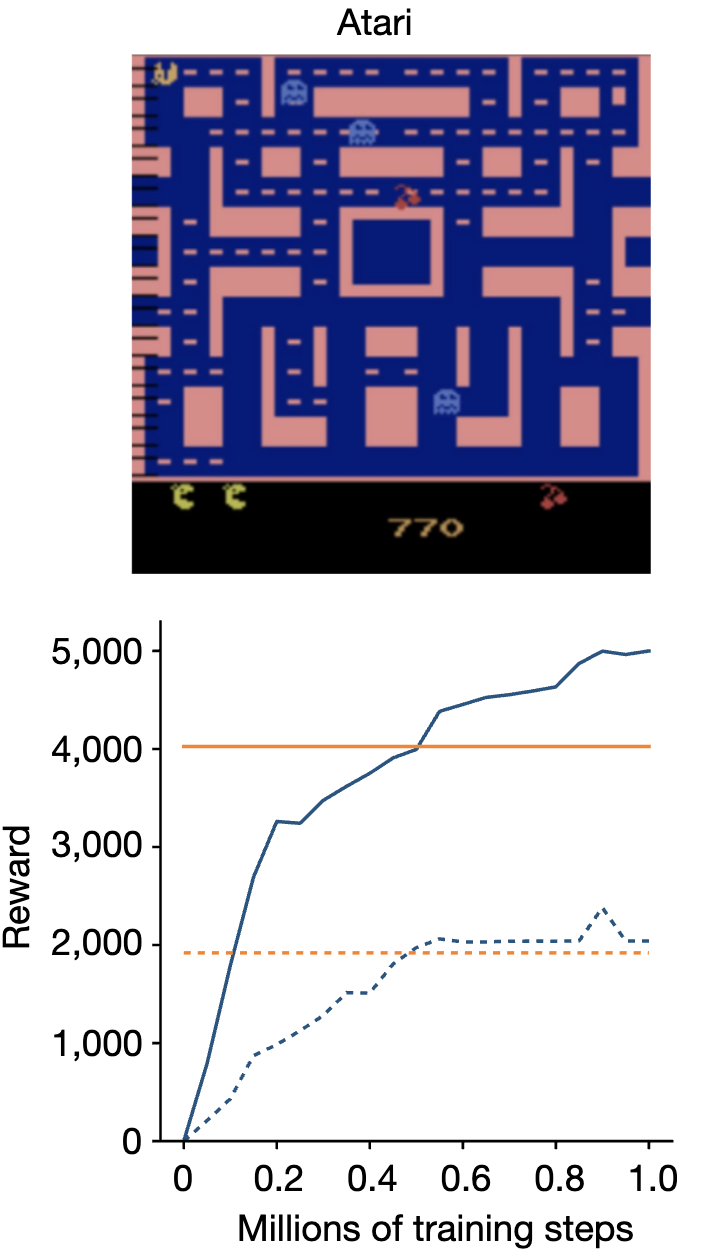
\includegraphics[height= 4.0in]{\images/muzeroatari}}

{\huge
  These are human normalized scores averaged over all 57 Atari games.  The orange line is the previous state of the art system.  Solid lines are average scores and dashed lines are median scores.
}

\slide{END}

}
\end{document}


